%!TEX root = ../main.tex

\section{Experimental design}

\label{sec:experimental-design}

In the previous section we suggest that emergent interfaces can make feature code change tasks (such as \textit{Scenario 1} and \textit{Scenario 2}) faster and less error prone. To evaluate these hypotheses and to get a better understanding of the benefits and drawbacks of emergent interfaces, we conducted and replicated a controlled experiment. We specifically investigate and compare code change effort and introduced errors when maintaining preprocessor-based product lines with and without our interfaces in a setting that supports virtual separation, allowing developers to hide feature code fragments.

\subsection{Goal, Questions, and Metrics}

Our evaluation aims to compare maintenance of preprocessor-based product lines with and without emergent interfaces (these are our treatments). Specifically, we are interested in the interaction with the feature hiding facilities of virtual separation of concerns, which we enable in both cases to aid comprehensibility. We evaluate emergent interfaces from the developer's point of view and observe effort and number of errors they commit. We investigate the following questions:

\begin{itemize}

	\item Question 1: \textit{Do emergent interfaces reduce effort during code change tasks involving feature code dependencies in preprocessor-based systems?}
	
	\item Question 2: \textit{Do emergent interfaces reduce the number of errors during code change tasks involving feature code dependencies in preprocessor-based systems?}

\end{itemize}

To answer Question~1 (effort), we measure the time required to find cross-feature dependencies and to change the impacted features to accomplish a code change task. Figure~\ref{fig:workflow-time} illustrates our setup with and without emergent interfaces.
Note that our setup does not measure the time needed to find the maintenance point (we actually provide the maintenance point with our task description as we describe below). While finding the maintenance point may dominate the entire tasks in a real-world setting, emergent interfaces do not contribute to that part. Hence, we measure only the part of the maintenance task after the maintenance point was identified. This focus of our measurement eliminates noise that would not contribute to our analysis. 

%We do not count the time to find the maintenance points. One might argue that the time to locate them is not negligible. However, given that our idea supports developers to better understand the impact of their changes, counting the time to locate such points would introduce bias to our evaluation. We claim we are still evaluating an important step of a maintenance task: the code change part. In other words, the implementation part. 

%In our experiments we measure only the implementation part of a maintenance task: the code change task (with or without emergent interfaces). This means we pre-select the maintenance points for the participants. One might argue that the time to locate the maintenance point is not negligible. However, measuring the time to find it would introduce bias. 

\begin{figure}[tp]
    \centering 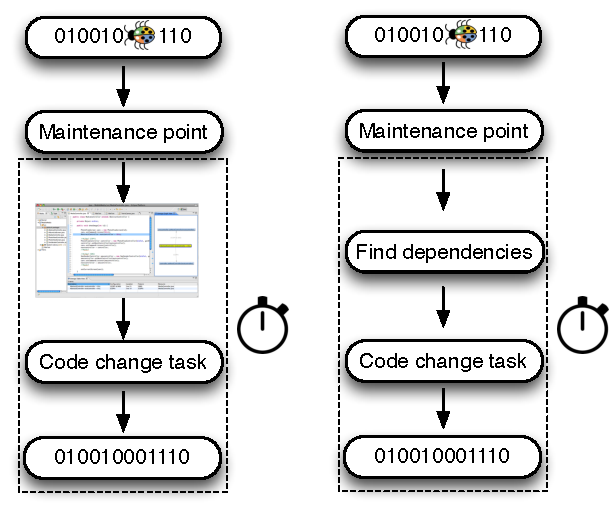
\includegraphics[width=0.35\textwidth]{images/Workflow-Time.pdf}
    \caption{Dashed rectangles represent the time we count (with and without emergent interfaces).}
    \label{fig:workflow-time}
\end{figure}

To answer Question~2 (correctness), we measure how many incorrect solutions the developer committed during a code change task (metric number of errors, or short NE). We consider error as a human action that introduces one or more defects to the code. 
As described below, for some tasks, we provide automated feedback to our participants, so the participant can retry after an incorrect attempt. Other tasks are evaluated manually after the experiment, so participants have only one attempt.

\subsection{Participants}

We performed the experiment in three rounds. In a first pilot study, we tested the experimental design with a small group of six graduate students at the University of Marburg, Germany. Next, we performed the actual experiment with 10 graduate students at Federal University of Pernambuco, Brazil (\textit{Round~1}). Finally, we replicated the experiment with 14 undergraduate students at Federal University of Alagoas, Brazil (\textit{Round~2}). In both rounds, around half of the participants had professional experience---varying from few months to many years of experience---and were actually part-time students. The 10 graduate students are attendants of a course on experimental software engineering lead by an independent lecturer. The 14 are UROP (Undergraduate Research Opportunity Program) students and volunteered to participate. All took part voluntarily and were informed they could stop participating at any time, but nobody did.

\subsection{Material and Code Change Tasks}

We use two preprocessor-based product lines as experimental material: \textit{Best Lap} and \textit{MobileMedia}. The former is a highly variant commercial product line that has approximately 15 KLOC. The latter is a product line for applications with about 3 KLOC that manipulate photo, music, and video on mobile devices~\cite{eduardo-empirical-study-icse08}. It contains feature restrictions and has been used in previous research studies~\cite{eduardo-empirical-study-icse08, rashid-ao-mm}.

We ask participants to perform a number of code change tasks in each of the product lines. Therefore, we provide the product line's source code and corresponding tasks that the participants should perform by modifying the source code. We selected tasks that are particularly affected by cross-feature dependencies, where we expect that our tool can contribute to a better understanding. Note that emergent interfaces target a specific class of problems; for other maintenance tasks we would not expect any benefit. We believe that our task selection can represent typical cross-feature problems as outlined in Section~\ref{sec:motivating}.

To cover different use cases, we prepare two kinds of tasks. In line with our motivating scenarios in Section~\ref{sec:motivating}, we distinguish between tasks where participants should implement a new requirement (requiring \textit{interprocedural} analysis of the existing source code) and tasks where participants should fix an unused variable (requiring only \textit{intraprocedural} analysis). We provide a task of each kind for each product line, for a total of four distinct tasks, as discussed in the following. All task descriptions are available online, see Appendix~A.

\paragraph{Task 1 - New requirement for Best Lap}

The new requirement for \textit{Best Lap} is similar to our motivating \textit{Scenario~1}, but differently from it, there are two methods of feature \textit{ARENA} that contain conditional statements forbidding negative scores. So, to accomplish the task, besides changing the \texttt{totalScore} assignment, participants should remove or rewrite these conditional statements (see one of them in method \texttt{setScore} of Figure~\ref{fig:arena-example}). To reach them, participants need to consider \textit{interprocedural} dependencies. That is, there are dependencies from the maintenance point to two conditional statements, each one in a different method.

In case Emergo is available, the participant should use it to identify the cross-feature dependencies between the variable \texttt{totalScore} and the rest of the code. Otherwise, the participant is free to use standard tools such as find/replace and  highlighting. This also holds for the subsequent tasks.

\paragraph{Task 2 - New requirement for MobileMedia}

The task for \textit{MobileMedia} is conceptually similar in the sense that participants should change a variable assignment, follow feature dependencies, and update conditional statements (here, only one \texttt{if} statement). However, differently from Task 1, where the method call depth to reach the two conditional statements is 1, here the call depth is 2. That is, from the maintenance point, we need to follow two method calls to reach the \texttt{if} statement.

%in that participants should change a variable and all dependencies (with or without Emergo). In \textit{MobileMedia}, participants should replace the actual address of a web server that delivered images with the address of a server that delivered different kinds of documents (including PDF files). The variable they should change is \texttt{server}. However, the change has a rippling effect that touches also upon the implementation of feature \emph{ZOOM}. Previously zoom functionality was only available for vector graphics, but should now also be supported for PDF files. Thus, to accomplish the task, participants should also update the \texttt{if} statement to take this new vector format into consideration. 

%\begin{table}[htb]
%\centering
%\footnotesize
%\begin{tabular}{|c|c|c|c|c|}
%\hline
% & \textit{\textit{Best Lap}} & \textit{\textit{MobileMedia}} \\
%\hline
%Fragments to change & 2 & 1\\
%\hline
%Method call depth & 1 & 2\\
%\hline
%Impacted feature & \textit{arena} & \textit{zoom}\\
%\hline
%Method LOC & 165 & 85\\
%\hline
%Number of Fragments & 4 & 5\\
%\hline
%Number of Features & 2 & 3\\
%\hline
%\end{tabular}
%\normalsize
%\caption{Summary of the \textit{New requirement} tasks characteristics.}
%\label{tab:m1-characteristics}
%\end{table}

\paragraph{Task 3 - Unused variable in Best Lap}

In \textit{Best Lap}, we asked participants to fix the unused-variable warnings for two variables: \texttt{tires} and \texttt{xP}. Such warnings are commonly found in many bug reports of preprocessor-based systems.\footnote{See \url{https://bugzilla.gnome.org/show_bug.cgi?id=461011}, \url{https://bugzilla.gnome.org/show_bug.cgi?id=167715}, \url{https://bugzilla.gnome.org/show_bug.cgi?id=401580}, \url{https://bugzilla.kernel.org/show_bug.cgi?id=1664}} We introduced the bugs ourself by removing correct \texttt{\#ifdef} directives around the variable declarations. We can solve all unused-variable tasks by following \textit{intraprocedural} dependencies only, but they typically require investigating code of different features. To accomplish the tasks, we ask participants to put a correct \texttt{\#ifdef} around the variable declarations. The variables \texttt{tires} and \texttt{xP} are inside methods with 147 and 216 source lines of code, respectively. 

\paragraph{Task 4 - Unused variable in MobileMedia}

Again the \textit{MobileMedia} task is conceptually similar to the \textit{Best Lap} task. Participants should fix the unused-variable warning of \texttt{numberOfViews} and \texttt{albumMusic}. The two variables are placed in shorter methods when compared to Task 3: they have 49 and 71 lines of code. The longest method here has less than half of the lines of the shortest one  in Task 3. 

Emergo computes dependencies for these tasks using \textit{def-use} chains based on the reaching definitions analysis. Thus, it points \textit{intraprocedural} and \textit{interprocedural} dependencies when maintaining a definition used by another feature.

Overall, the tasks for both product lines have similarities, but they are not equivalent. Actually, these differences---methods size, method call depths to reach the impacted feature, and number of conditionals to change---between task for both product lines help us to better analyze the effects of our two treatments and is properly controlled by our experiment design, as we shall see in Section~\ref{sec:design}.

%\reviewer{On what basis do you believe they are comparable? Were they of comparable difficulty to the participants in the study?}

%\reviewer{(I have added a paragraph on this above and we should discuss this in 5.3, otherwise we are fine) Second, I do not mind that the tasks used were simple in nature, however, I do think the type of tasks (the types of changes that were required) were extremely skewed to show the benefits of the tool. It is not realistic to evaluate a tool that highlights hidden dependencies using a scenario where the variable that has the hidden dependencies has been pre-selected for the developers. I would contend that these tasks are by no means representative of real tasks, even small ones.}

Finally, we designed warmup tasks on a toy product line so that participants could learn how to generate emergent interfaces using Emergo at the start of the experiment. We perform warmup tasks together in a class context and are not evaluated.

\subsection{Hypotheses}

Based on our goals and tasks, we evaluate the following hypotheses:

%When using emergent interfaces, developers are aware of features dependencies. This might lead them to find dependencies quickly and, consequently, they can accomplish the task faster.
\begin{itemize}

	\item \textit{H1 - Effort:} With emergent interfaces, developers spend less time to complete the code change tasks involving feature dependencies in both product lines.

%Since developers are aware of dependencies, the probability of changing the impacted features increases, leading them to not submit incomplete tasks.
	\item \textit{H2 - Error introduction:}  With emergent interfaces, developers commit less errors in both product lines when performing the code change tasks involving feature dependencies.

\end{itemize}

\subsection{Design}

\label{sec:design}

To evaluate our research questions, we distinguish between participants using our treatments (independent variable with two levels: with and without emergent interfaces). Additionally, we distinguish between the tasks of both product lines, as we cannot assume equivalence (independent variable with two levels: \textit{Best Lap} and \textit{MobileMedia} tasks). We measure time and the number of errors (dependent variables) for new-requirement tasks and unused-variable tasks.

Since we have two independent variables with two levels each, we use a standard \emph{Latin Square design}~\cite{box-statistics-for-experimenters}. We randomly distribute participants in rows and product lines tasks in columns. The treatments come inside each cell. Each treatment appears only once in every row and every column (see Figure~\ref{fig:latin-squares}). As a result, each participant performs both kinds of tasks on each product line and also uses and not uses emergent interfaces at some part of the experiment, but no participant will perform the same task twice, which avoids corresponding carry-over effects, such as learning (if we let one to use both treatments in the same task, we would favor the second treatment, since she already knows how to accomplish the task). The design does not favor any treatment and blocks two factors: participant and code change tasks.

\begin{figure}[tp]
    \centering 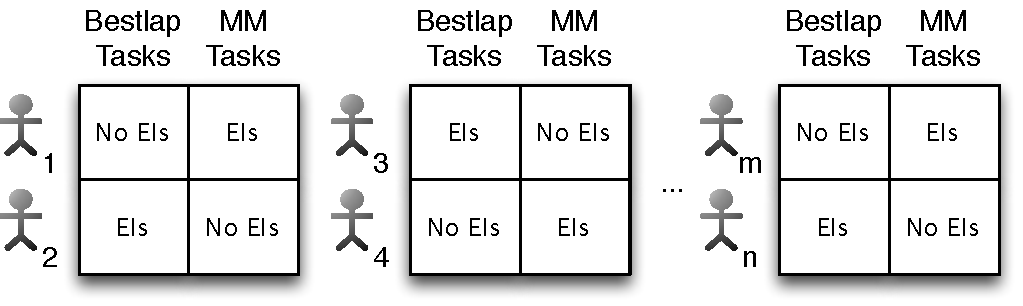
\includegraphics[width=0.48\textwidth]{images/Latin-squares.pdf}
    \caption{Layout of our experiment design: Latin squares.}
    \label{fig:latin-squares}
\end{figure}

As analysis procedure for this design, we perform an analysis of variance (ANOVA). The test compares the effect of the treatments on the dependent variables. To give relevance to the ANOVA~\cite{box-statistics-for-experimenters}, we use the Bartlett, Box Cox, and Tukey tests to verify variance homogeneity, normal distribution, and model additivity, respectively. We follow the convention of considering a factor as being significant to the response variable when \textit{p-value} $< 0.05$~\cite{box-statistics-for-experimenters}.

\subsection{Procedure}

After randomly assigning each participant into our Latin Square design, we distribute task description sheets accordingly. Each participant performs two tasks in two individually prepared installations of Eclipse (with Emergo installed or not, with \textit{Best Lap} or \textit{MobileMedia} prepared readily as a project); each installation corresponds to a cell of our Latin Square design. By preparing the Eclipse installation, we prevent participants from using Emergo when they are not supposed to (it is simply not installed in that case). All Eclipse installations support virtual separation, where we leave the first line with the \texttt{\#ifdef} statement to inform the user of hidden code). Also for the warmup tasks, we prepared a distinct Eclipse installation.

%We randomly assign each participant to form four groups for our Latin Square design and distributed tasks specific sheets corresponding to the groups. Each group performs 

All tasks focus around a specific variable. Since we are not interested in the time needed to locate the variable, we prepare the installations in such a way that the correct files are opened and the cursor is positioned exactly at the maintenance point.

%\reviewer{Third, the authors explicitly ignore in their experiments the time required to locate the variable. The time and effort required to locate a bug is by no means negligible, and even if this time is of no interest to your experiment, reducing a maintenance task to modifying a variable whose location is known is, in my opinion, not a valid simplification of any real maintenance task.}

%Notice that all tasks target variables. To avoid counting time to search for these variables and allow participants to focus directly on the tasks, we save all Eclipse workspaces in such a way that, when opening them, the classes that contain the variables are already open. Also, the Eclipse editor cursor already points to the target variable of each class we consider.

We prepare all Eclipse installations with an additional plug-in to measure the times automatically. The plug-in adds two buttons: a \textit{Play/Pause} button for participants to start/stop the chronometer; and a \textit{Finish} button to submit a solution. We instruct the participants to press \textit{Play} when starting with the task after reading its description and \emph{Finish} when done, and to use \emph{Pause} for breaks (for asking questions during the experiment, for example). To collect qualitative data, in the pilot study we also recorded the screen.

To illustrate the tasks from the participant's perspective, we summarize in Figure~\ref{fig:maintenance-tasks} the task description sheets we distributed. We represent the steps that participants should follow as ``a", ``b", and ``c". Notice that we associate each sheet with a different Eclipse instance.

We also partially automated measuring the number of errors. For new-requirements tasks (Tasks 1 and~2), the plug-in automatically checks the submitted solution by compiling the code and running test cases (require about 1 second), as soon as the participant presses \emph{Finish}. If the test passes, we stop and record the time, otherwise we increase the error counter and let the participant continue until the test eventually passes. The test cases are not accessible to the participants. For unused-variable tasks (Tasks 3 and~4) we do not provide immediate feedback but evaluate after the experiment whether one or both variables are correctly fixed. This is because we learned (when watching the pilot screen recordings) that participants spend time dealing with compilation errors regarding missing \texttt{\/\/\#endif} statements and tokens like ``//" and ``\#". Because we do not want to measure this extra time, we ask participants to write the \texttt{\#ifdef} feature expression in the task description sheets. For example, to fix the unused variable illustrated in Section~\ref{sec:breaks}, they can write ``\texttt{CHOWN || UTIMES}" in the sheet.

\begin{figure}[tp]
\centering
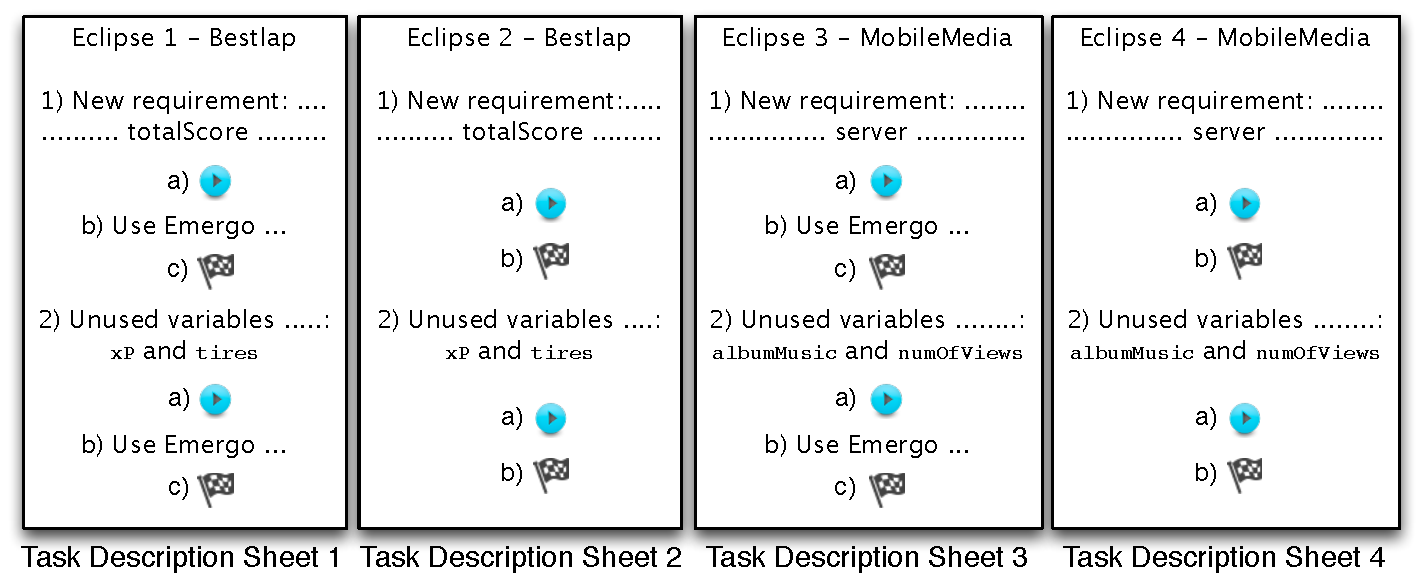
\includegraphics[width=\linewidth]{images/Maintenance-Tasks.pdf}
\caption{Task description sheets we distributed to the participants.}
\label{fig:maintenance-tasks}
\end{figure}

%\reviewer{As you point out the time penalty approach you use is rather arbitrary. While I can mostly accept your argument, I am less clear on why you chose to count number of errors for the unused variable task when participants were unable to test their results. This difference between using tests with the new requirements task and not having tests with the unused variables means the participants have a very different experience with each kind of task in using the emergent interfaces. I think the lack of tests for the unused variable tests moves far enough away from actual development that I do not think your results are very meaningful. The combination of the time penalty approach and the counting of errors without tests makes it unclear to me that the overall results of your experiments have sufficient validity.}

All times using emergent interfaces \textit{include} the time required by Emergo to compute these interfaces. Emergo takes, on the used systems, around $13$ seconds and $6$ seconds to generate emergent interfaces for Tasks 1 and~2, respectively. To compute interfaces for Tasks 3 and~4, we only need \textit{intraprocedural} analyses,  but, to simplify execution, instead of asking the developers to select the analysis to use, we let Emergo automatically apply \textit{interprocedural} ones. So, instead of 1 second or less (\textit{intraprocedural} analyses), it takes more time than needed, around 11, 16, 2, and 3 seconds for the variables \texttt{tires}, \texttt{xP}, \texttt{numberOfViews}, and \texttt{albumMusic}, respectively.

%However, notice that to compute emergent interfaces for the \textit{Unused variable} task, we do not need \textit{interprocedural} analyses. But to reduce complexity and thus avoid errors during the experiment, we do not ask developers to switch from \textit{interprocedural} to \textit{intraprocedural} analyses. So, Emergo generates all interfaces based on \textit{interprocedural} analyses, meaning that it spends more seconds than needed (when considering \textit{intraprocedural} analyses, Emergo takes around $1$ second or less).

To avoid the effect of software installed in different machines and related confounding parameters, we conduct the experiment in a virtual machine (executed on comparable hardware) that provides the same environment to all participants. All participants worked on the same time in the same room under the supervision of two experimenters.

%Each group uses a differently prepared version of Eclipse with or without emergent interfaces installed and with a prepared workspace for the Best Lap or MobileMedia task:
%\begin{itemize}
%
%	\item \textit{Eclipse 1:} Emergo installed; \textit{Best Lap} imported;
%	\item \textit{Eclipse 2:} Emergo not installed; \textit{Best Lap} imported;
%	\item \textit{Eclipse 3:} Emergo installed; \textit{MobileMedia} imported;
%	\item \textit{Eclipse 4:} Emergo not installed; \textit{MobileMedia} imported.
%
%\end{itemize}

%Providing these $4$ Eclipses aims to reduce problems during the experiment execution. For example, if we provide only one Eclipse with everything, the participant can use the wrong technique in the wrong SPL. Notice that each Eclipse represents one cell of our latin square design. We also have an additional Eclipse with Emergo installed and a toy SPL imported (\textit{JCalc}, a simple calculator) for the experiment dry-run.

%To understand the participants behavior, we recorded their screens in the \textit{Pilot} execution. We learned that they commit errors regarding tokens and statements such as ``//", ``\#", ``(" expression ``)", or \texttt{\#endif}, leading to many compilation errors. Since participants waste time dealing with these errors, they rather write the feature expressions in the task description sheets. Hence, the \textit{Unused variable} task does not have test cases. Again, in case Emergo is available, participants should use it. They also press \textit{Play} after reading the \textit{Unused variable} task.

%To form the latin squares, we randomly allocate participants to squares, then for each square we apply a different randomization to allocate treatments to each cell. After the randomization for all participants, we distribute the task sheets accordingly.

\subsection{Executions and Derivations}

At the start of the experiment session, we introduce preprocessors, the hiding facilities of virtual separation of concerns, and emergent interfaces. Together with the participants, we perform a warmup task that uses Emergo. We introduce how to use the \emph{Play/Pause} and \emph{Finish} buttons. For the entire experiment, we scheduled 2.5 hours (training, warmup, and execution). No deviations occurred.

%To make participants aware of preprocessors, VSoC, feature dependencies, emergent interfaces, and Emergo, we provide training before running the experiment, which takes around $1$ hour. Our idea consists of providing a minimum knowledge so that all participants can accomplish all tasks.
%We explain how to compute emergent interfaces using Emergo and how to navigate throughout the code using it. Then, we explain the buttons \textit{Play/Pause} and \textit{Finish}. We also discuss the target SPLs but we do not present any code of them. Finally, we inform they sometimes use Emergo and sometimes do not.

%After training, we distribute \textit{New requirement} and \textit{Unused variable} tasks based on the \textit{JCalc} toy SPL. Then, we execute a dry-run simulating the experiment, so participants use Emergo, projections that implement the VSoC idea, and the buttons exactly as if they are executing the experiment for real.
